%% This document gives an example on how to use the gucmasterthesis
%% LaTeX document class.

%% Use short name MMT MIS or CIMET, and language,  english or norwegian
\documentclass[MACS,english]{gucthesis}

\usepackage[T1]{fontenc}
\usepackage[utf8]{inputenc}     % For utf8 encoded .tex files allows norwegian characters in the files. This can be dangerous if you change to a differnt editor.
\usepackage[pdftex]{graphicx, hyperref}   % For cross references in pdf
\usepackage{color}              % For colouring text   
\usepackage{url}

\begin{document}

\thesistitle{Example Masters Thesis. With a long title to test the wrapping of the box}
\thesisauthor{Simon McCallum}
\thesissupervisor{Nils Kalstad Svendsen}
%\thesissupervisorA{Jon Yngve Hardeberg}  % if you have a second supervisor add it like this
\thesisHostInstitution{\GUC}

%\thesisHostInstitution{University of Eastern Finland}

%\thesisjuryA{} %jury names
%\thesisjuryB{} %jury names
%\thesisjuryC{} %jury names
%\thesisjuryD{} %jury names

\gmtkeywords{Thesis, Latex, Template, IMT}
\gmtdesc{This is the short description of a masters thesis}


\thesisdate{\gucthesisdate}
\useyear{2012}


 % this is the file which contains all the details about your thesis
\makefrontpages % make the frontpages
\thesistitlepage % make the ordinary titlepage

\chapter*{Abstract}

This document provides an example on how to use the
\texttt{gucthesis} \LaTeX\ class that has been developed in
order to fulfil the typographical requirements for the master's and bachelor's thesis
at \GUC.

%\include{summary}

\chapter*{Preface}

I would like to thank Erik Hjelm\aa{}s for encouraging me to write this
small \LaTeX\ class for GUC's master's theses \dots




\tableofcontents

% Comment with a percent to remove figures or tables:
\listoffigures
\listoftables


\chapter{Introduction}
\label{chap:introduction}



\section{Topic}
Task and time management applications help users stay organized by keeping track of notes, meetings, tasks etc. Many applications exist that are directed towards this purpose, ranging from simple note-taking applications and to-do lists to more advanced ones like calendars and scheduling applications. A calendar typically holds events or appointments for a user while a to-do list will keep more detailed and lower level tasks. All of these applications have in common that they relieve the user of having to remember things, thus allowing the user to focus more deeply on other things.

Context awareness is also a field of research that has received more attention in recent years. The reason for this is the increasing number of mobile devices that are available and also the increasing functionality of these devices. When it comes to context awareness, the sensors in mobile devices play a huge role. There are more sensors packed into these devices now than ever before, which allows applications to collect very specific types of contextual information. This in turn allows for the development of applications that have very specific and tailored purposes.

By combining context awareness and task management, we open up for new types of applications. Smarter systems could be built that leverage contextual information, both past and present, to adapt its behavior to accommodate very specific situations. A calendar system for example, could evaluate a user's upcoming meeting and the current location of the user. Taking into account the distance between the user and meeting location, the system could then deliver a reminder at the appropriate time, allowing the user to catch the meeting. Another example would be a to-do list application that could leverage contextual information about previously performed tasks to provide task recommendations to the user.





\section{Problem description}
Task and time management applications are valuable tools that are used by many people. These applications can be especially valuable on mobile devices as the users can carry these devices with them, thus having the application data easily accessible. Concrete and popular examples of such applications are calendars such as Google Calendar\cite{googlecalendar} or to-do list applications such as Trello\cite{trello} or Todoist\cite{todoist}. Even though these, and many similar applications are very useful, their functionality and usefulness could be further improved by integrating user context. 

Utilization of contextual information in different scenarios have been widely researched. However, we have found no research that studies the usage of such information in the specific domain of task and time management systems. Many systems are improved by making them context-aware. One example of this is Learning Management Systems (LMS) that can suggest learning content based on the users current context\cite{verbert2012context}, and in doing so increasing the level of learning for the user. Following examples such as this, it is believed that task management applications can also reap the benefits of context awareness.

This study will look into the area of utilizing contextual information in task management applications. We will design a proof of concept application that tries to make use of the user's contexts.

\section{Justification, motivation and benefits}
The complete envisioned application is a personal information manager (PIM) where the user only needs to inform the application of the tasks that he/she needs to perform. The application would then suggest a current task and provide an optimal ordering of the other tasks, taking into account the current user context. This optimization can for example be based on minimizing total time spent completing the tasks, minimizing total travel distance between tasks, thereby reducing travel costs and pollution, or a combination of these. With respect to time, this would mean that completing the tasks in any other order than that suggested by the system would lead to a longer time spenditure. In order to create such a system, many areas would need extensive research, more than that which is possible to complete within the scope of this thesis. However, sub-parts of the system can be identified and researched, providing building blocks for the realization of the entire system. These sub-parts include how to collect relevant context data, how to store those data, how to implement an overall design of such an application and how to evaluate past tasks and contexts to successfully produce task suggestions. Identifying and researching these parts of the system justifies the work to be conducted in this thesis, as it allows for working towards the higher-end goal. The motivation behind the thesis is to be able to contribute to to-do applications, and by extension task management applications in general, by further enhancing their task management capabilities.



\section{Research questions}

This thesis is three folded. Firstly, there is the area of context collection and representation. Secondly, we have the software engineering area, which relates to application design and functionality. The third area revolves around the context in which the previous two are placed for this thesis, namely students and the educational context for which the thesis is conducted in. The proposed solution will have to address all of these areas in detail. Therefore, these research questions have been formed for each of the areas:
\begin{itemize}
	\item \textbf{Research question 1}: What contexts are relevant in a task management application, and how can they be acquired and modeled?
	\item \textbf{Research question 2}: How can a task management application be designed and what are the important design decisions when making such an application?
	\item \textbf{Research question 3}: How can context information be utilized in a task management application?
\end{itemize}

\section{Thesis structure}
Chapter~\ref{chap:relatedwork} provides the necessary background that related to the work in this thesis. State-of-the-art task management applications are also covered here. Chapter~\ref{chap:methodology} describes the whole process of designing the to-do list application and is also in its entirety the answer to research question 2 and 3. Chapter~\ref{chap:results} presents the findings in this thesis and is together with Chapter \ref{chap:methodology} and \ref{chap:discussion} the answer to research question 1. Chapter~\ref{chap:discussion} discusses the different approaches and decisions made in this thesis, as well as discussing alternatives for some of these decisions. The work is then concluded in Chapter~\ref{chap:conclusion} and futer work is discussed in Chapter~\ref{chap:futurework}. % includes latex files from the same directory
\chapter{Packages}
\label{chap:packages}

The \texttt{gucthesis} is built upon the standard \LaTeX\
\texttt{report} class. All commands from the \texttt{report} class can
be used, with the two exceptions of \verb+\subsubsection+ and
\verb+\paragraph+. This is because there should only be three
levels of headings according to the guidelines~\cite{GUCMaster}.

\section{Packages Used by gucthesis}
\label{sec:packages}

In addition to the \texttt{report} document class,
\texttt{gucthesis} makes direct use of the following packages
that must hence be present:
\begin{description}
	\item[geometry:] used for setting the sizes of the margins and
  	headers.
	\item[fontenc:] used with option \texttt{T1} for forcing the Cork font
  	encoding (necessary for the Charter font).
	\item[charter:] load Charter as the default font.
	\item[euler:] load the Euler math fonts.
	\item[bable:] for language handling.
\end{description}

\section{Other Relevant Packages}
\label{sec:otherpackages}

The author of a thesis might want to use a bunch of different packages
to those described in Section~\ref{sec:packages} in order to have all features needed for their document. 
In particular, it is advised to use the following:
\begin{description}
	\item[inputenc:] to allow \LaTeX\ to use more than 7-bit ASCII for its
	  input. Most often, the option \texttt{latin1} will do.
	\item[babel:] to load language specific strings. Reasonable options
	  include \texttt{british}, \texttt{american}, \texttt{norsk} and
	  \texttt{nynorsk}.
	\item[graphicx:] to include graphics.
	\item[hyperref:] this is a very nice package that makes cross links in
	  pdf documents. Use with option \texttt{dvips} or \texttt{pdftex}
	  in accordance with the driver that you use. Unfortunately, hyperref
	  is not completely bugfree\dots
\end{description} % could be called Methodology or methods or anyfile name 
\chapter{Structural Elements}
\label{chap:structural}

The title of the thesis should be set using the \verb+\thesistitle+
command, and the date of the thesis should be set using the
\verb+\thesisdate+ command. This makes the title and date appear in
the running header, like in this document.

\section{Page Layout}

The geometry of the page has been set using the \verb+\geometry+
command.

\section{Fonts}

Due to limited \LaTeX\ support for the Georgia font, Charter has been
chosen instead. For mathematical formula, the Euler fonts are used,
since they blend more nicely with the Charter than the standard
\LaTeX\ fonts: 
$$
 f(x) = \int_0^x g(\tau)\,d\tau
$$

For inline math you can use $\backslash{}($ and $\backslash{})$ for example \( f(x)= \frac{x^2}{1+x^2} \).  
This also allows you to use $\slash$ and $\backslash$. You need to include the \{\} when you want the special
character to have other letters immediately after it.

\section{Sectioning Commands}

The standard \LaTeX\ sectioning commands are used for both numbered
and unnumbered sections. The top level is given by the \verb+\chapter+
command. This starts a new right page. The two lower levels are
obtained using the \verb+\section+ and \verb+\subsection+ commands.
The standard \LaTeX\ \verb+\subsubsection+ and \verb+\paragraph+
commands have been disabled since their use is not encouraged by the
thesis guidelines. When you use these they will not be given numbers.  
They still appear in the document with highlighting but not in the 
table of contents.

\subsection{The subsection}

This is an example of a subsection.

\subsubsection{The subsubsection}

This is an example of a subsubsection.

\paragraph{The paragraph}

This is an example of a paragraph with a heading.

\section{Floats (Figures and Tables)}
\label{sec:floats}

Figures are placed in the \texttt{figure} environment. An example is
shown in Figure~\ref{fig:example}. %notice the ~ in between figure and the \ref. it stops latex from splitting the number and word over a line.
Tables are placed in the \texttt{table} environment. An example is given in
Table~\ref{tab:example}. Figures and tables float freely around in the
document in accordance with standard \LaTeX\ behavior.

\begin{figure}[tbp]  %t top, b bottom, p page | you can also use h to try to get the figure to appear at the current location
  \centering
  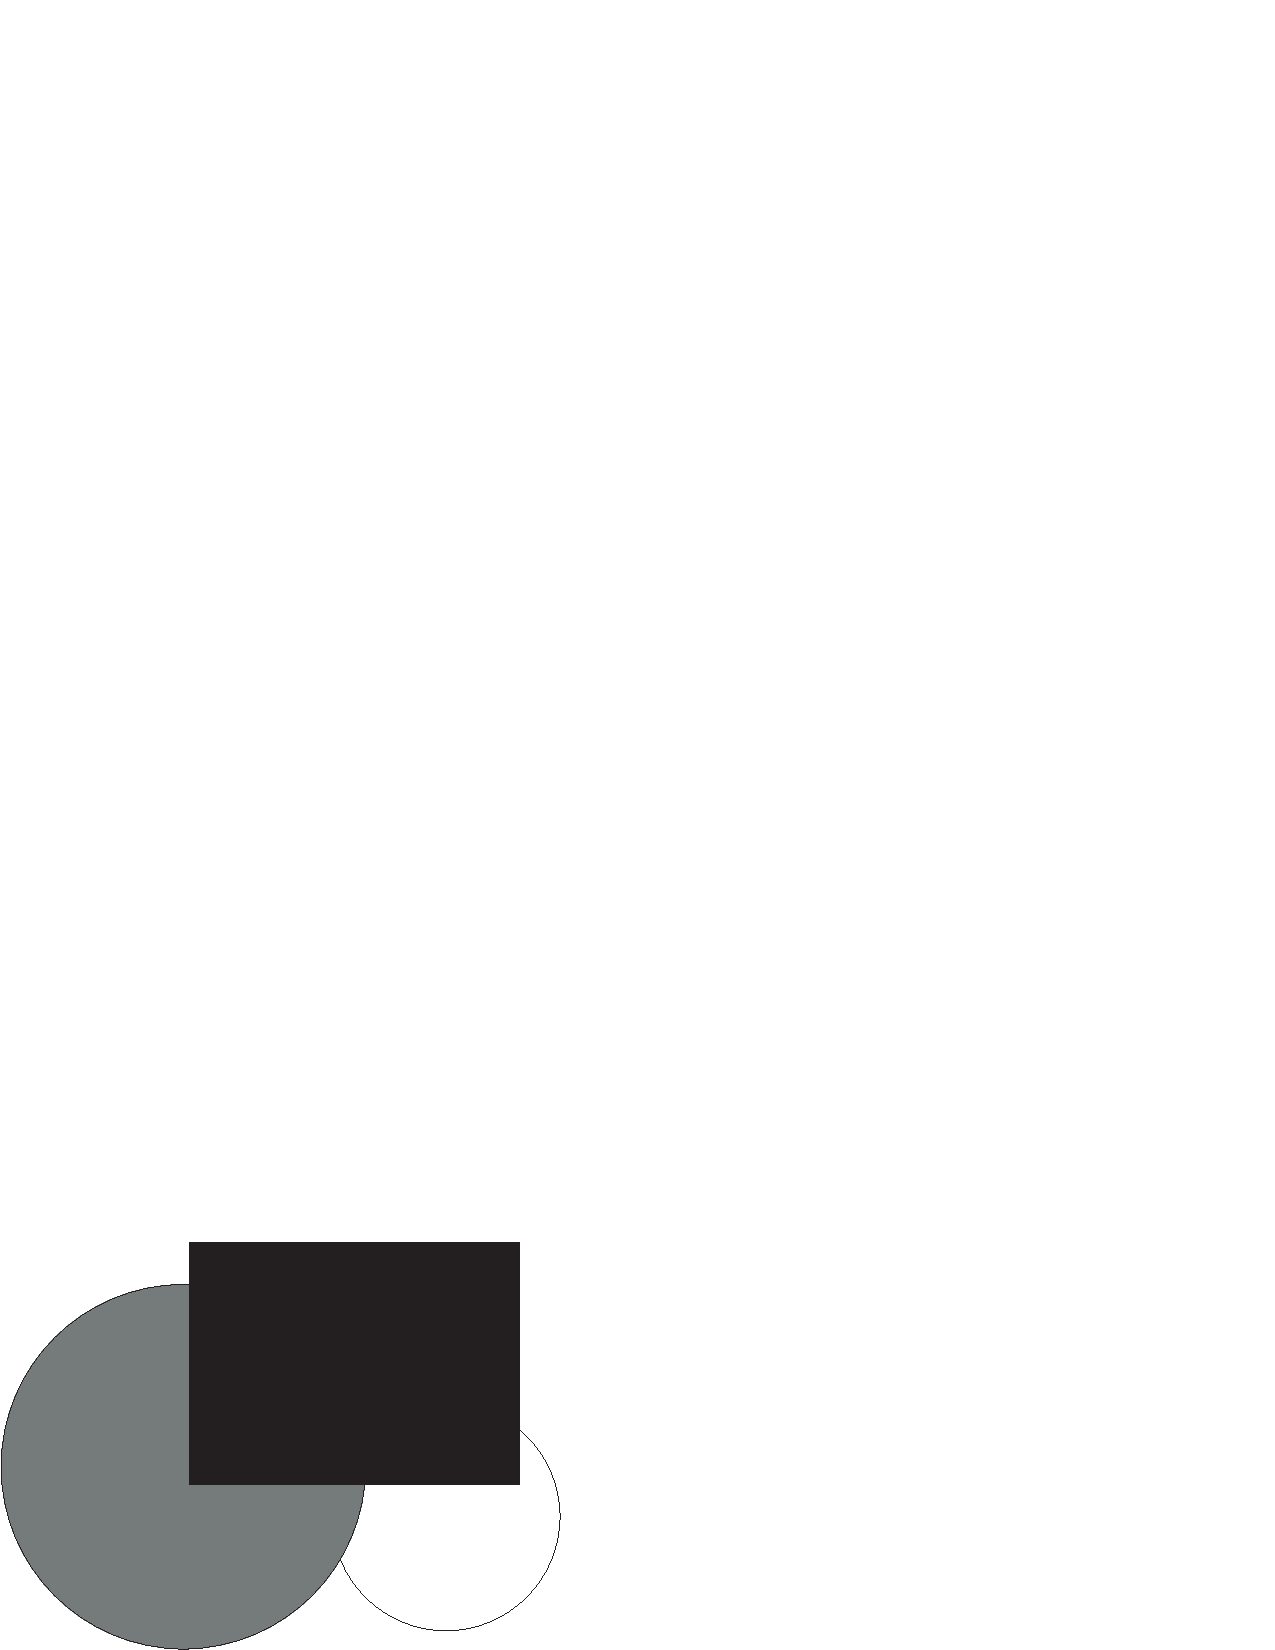
\includegraphics[width=.5\textwidth]{example_fig}
  \caption[An example figure.]{An example figure. If the caption is
    shorter than one line, it is centered. If it goes over more than
    one line, it is left and right justified. Furthermore, it is
    suggested that an alternative short caption is given in order to
    produce a good list of figures.}
  \label{fig:example}
\end{figure}

\begin{table}[tbp]
  \centering
  \begin{tabular}{c|c}
    Age  & IQ  \\ 
    \hline
    10   & 100 \\
    20   & 100 \\
    30   & 150 \\
    40   & 100 \\
    50   & 100
  \end{tabular}
  \caption{An example table.}
  \label{tab:example}
\end{table}

The captions are placed \emph{below} both for the figures and the
tables. The caption is set in 9pt. If the caption is shorter than one
line, it is centered.

\section{Quotes}
\label{sec:Quotes} % this allows you to refer to this section number using \ref{sec:Quotes}

Quotes are inserted using the standard \LaTeX\ \texttt{quote}
environment. The environment has been changed so that a 9pt font is
used:

\begin{quote}
  ``And I looked, and, behold, a whirlwind came out of the north, a
  great cloud, and a fire infolding itself, and a brightness was about
  it, and out of the midst thereof as the colour of amber, out of the
  midst of the fire. Also out of the midst thereof came the likeness
  of four living creatures.''
\end{quote}

\section{Lists}
\label{sec:lists}

Point lists and enumerated lists are made by using the standard
\texttt{itemize} and \texttt{enumerate} environments, respectively.
The spacing is going to be changed in accordance with the specification. For
\texttt{itemize}, the results look like this:
\begin{itemize}
	\item First item.
	\item Second item. Here I will put some long text, just to illustrate.
	  Here I will put some long text, just to illustrate. Here I will put
	  some long text, just to illustrate. Here I will put some long text,
	  just to illustrate.
	\item Third item also has subitems:
	  \begin{itemize}
		  \item First subitem.
		  \item Second subitem.
		  \item Third subitem.
	  \end{itemize}
\end{itemize}
and for \texttt{enumerate} like this:
\begin{enumerate}
	\item First item.
	\item Second item. Here I will put some long text, just to illustrate.
	  Here I will put some long text, just to illustrate. Here I will put
	  some long text, just to illustrate. Here I will put some long text,
	  just to illustrate.
	\item Third item also has subitems:
	  \begin{enumerate}
		  \item First subitem.
		  \item Second subitem.
		  \item Third subitem.
	  \end{enumerate}
\end{enumerate}

You may also want to use descriptive lists
\begin{description}
	\item[First] the first item.
	\item[Second] the second item. Here I will put some long text, just to illustrate.
	  Here I will put some long text, just to illustrate. Here I will put
	  some long text, just to illustrate. Here I will put some long text,
	  just to illustrate.
	\item [What now] the third item also has subitems:
	  \begin{enumerate}
		  \item First subitem.
		  \item Second subitem.
		  \item Third subitem.
	  \end{enumerate}
\end{description}


\section{Bibliographic References}

You should cite articles~\cite{Askvall1985}, books~\cite{Card1983},
anthologies~\cite{Lancaster1985} and web publications~\cite{Meldon1997}
like this. There is always an issue referencing web pages. Currently
we suggest that you use the HiG Website~\cite{HiG:Website}.


A particular bibliography style file for GUC named
\texttt{gucthesis.bst} has been developed based upon the
standard Bib\TeX\ \texttt{unsrt} style.
 % could be results



\bibliographystyle{gucthesis}
\bibliography{MastersExample}

\appendix
\section{Student tasks questionnaire}

\begin{figure}[tbp]
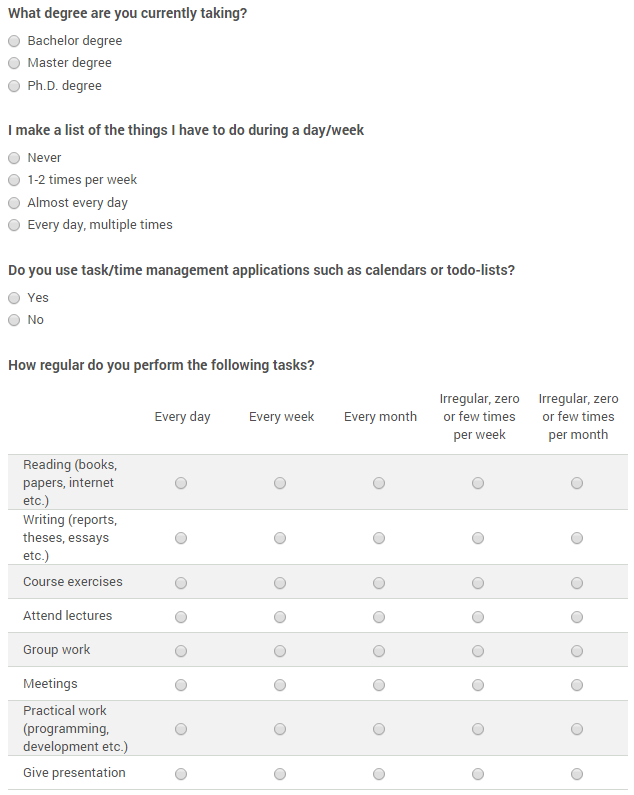
\includegraphics[width=\columnwidth]{appendix/StudentTasks1.PNG}
\caption{}
\label{}
\end{figure}

\begin{figure}[tbp]
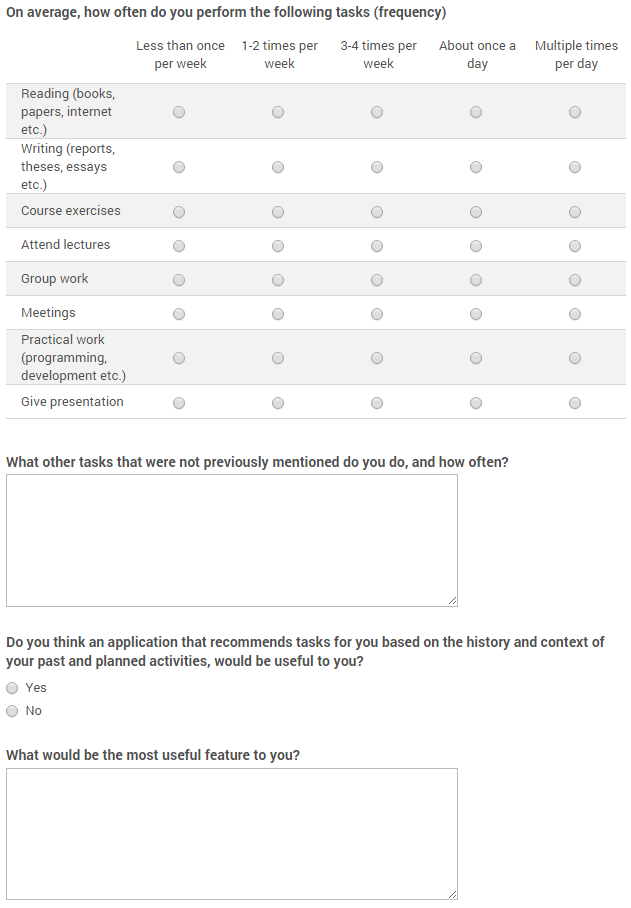
\includegraphics[width=\columnwidth]{appendix/StudentTasks2.PNG}
\caption{}
\label{}
\end{figure}

\end{document}
